% Created 2018-03-17 Sat 00:08
\documentclass{article}
\usepackage[mathletters]{ucs}
\usepackage[utf8x]{inputenc}
\usepackage[T1]{fontenc}
\usepackage{fixltx2e}
\usepackage{graphicx}
\usepackage{longtable}
\usepackage{float}
\usepackage{wrapfig}
\usepackage{rotating}
\usepackage[normalem]{ulem}
\usepackage{amsmath}
\usepackage{textcomp}
\usepackage{marvosym}
\usepackage{wasysym}
\usepackage{amssymb}
\usepackage{hyperref}
\tolerance=1000
\usepackage[margin=1.0in]{geometry}
\date{\today}
\title{Notebook3}
\hypersetup{
  pdfkeywords={},
  pdfsubject={},
  pdfcreator={Emacs 25.3.1 (Org mode 8.2.10)}}
\begin{document}

\maketitle
\tableofcontents

\section{Comparing the Convolution to the Transform}
\label{sec-1}
\begin{itemize}
\item Section 3.4 in the book describes that the due to how the math works
out multiplication in Fourier space $F(ω)H(ω) = f(x)*h(x)$ where F(ω) and
H(ω) are the Fourier transform on f(x) and h(x) respectively.
\item For my tests Ι have also compared the convolution to multiplication
in Cosine Transform space, which lead to interesting results.
\end{itemize}
\section{Implementation of the test}
\label{sec-2}
\begin{itemize}
\item Since Ι did tests with both the cosine and fourier transformers,
Notebook2 has the filters for dct which won't be reposted.
\item At first I wasn't sure how to convert a Double into a ℂ number, so I
only tested the dct first, however I later figured out that I can
just set the imaginary number to 0 for images.
\begin{verbatim}
repaFft :: Shape sh ⇒ Array V sh Double → Array V sh (ℂ Double)
repaFft = repaVecComp (fft . fmap (:+ 0))

repaIFft :: Shape sh ⇒ Array V sh (ℂ Double) → Array V sh Double
repaIFft = repaVecComp (fmap magnitude . ifft)

repaFftP :: (Monad m, Load r sh Double) ⇒ Array r sh Double → m (Array V sh (ℂ Double))
repaFftP = fmap repaFft . computeVectorP

repaIFftP :: (Monad m, Load r sh (ℂ Double)) ⇒ Array r sh (ℂ Double) → m (Array V sh Double)
repaIFftP = fmap repaIFft . computeVectorP
\end{verbatim}
\begin{itemize}
\item When converting an image to fft, we just add 0 to the imaginary
part, and when we compute the inverse, we just take the magnitude,
safely converting the image back into a Double from being Complex.
\end{itemize}

\item Besides the above function for FFT transforms, Ι noticed that after
running my tests the image was off by around 3 pixels (not 2 but not
quite 3 actually), so the below function was made
\begin{verbatim}
offsetFft :: Source r b ⇒ Array r DIM2 b → Array D DIM2 b
offsetFft arr = R.traverse arr id f
  where sh@(Z :. i :. j) = extent arr
        f index (Z :. x :. y)
          | isInside2 sh newShape = index newShape
          | x + 2 ≥ i ∧ y + 2 ≥ j = index (ix2 (x + 2 - i) (y + 2 - j))
          | x + 2 ≥ i             = index (ix2 (x + 2 - i) (y + 2))
          | otherwise             = index (ix2 (x + 2)     (y + 2 - j))
         where newShape = ix2 (x + 2) (y + 2)
\end{verbatim}
\begin{itemize}
\item This code just creates a new array where all the pixels are shift
down and right by two and wrap around when encountering an edge.

\item this code can easily be made more general instead of shifting
everything by 2 you pass in a pad down and a pad up.
\end{itemize}

\item Now that we have all the transformers we need, we can start to make
our filters and padding our filters.
\begin{verbatim}
-- the one given in the python code is wrong, as it uses [1,2,6,2,1]
-- it seems even the lecture is wrong, because if yo add them all up, they
-- don't add up to 256.. can check by summing over my gausian and seeing its 256
gausian :: Array U DIM2 Double
gausian = fromListUnboxed (ix2 5 5) $ (*) . (/ 256) <$> [1,4,6,4,1] <*> [1,4,6,4,1]
\end{verbatim}
\begin{itemize}
\item Here we create the 5 by 5 Gaussian filter array by using the
generalized cross product trick from Notebook1, then transforming
the list into an array
\end{itemize}
\begin{verbatim}
pad :: (Source r e) ⇒ e → DIM2 → Array r DIM2 e → Array D DIM2 e
pad val sh vec = fromFunction sh makePad
  where
    Z :. i :. j = R.extent vec
    makePad sh@(Z :. x :. y)
      | x ≥ i ∨ y ≥ j = val
      | otherwise     = vec ! sh

padOff :: (Source r e) ⇒ e → DIM2 → Array r DIM2 e → Int → Int → Array D DIM2 e
padOff val sh vec offx offy = fromFunction sh makePad
  where
    Z :. i :. j = R.extent vec
    makePad sh@(Z :. x :. y)
      | x - offx ≥ i ∨ x - offx < 0
      ∨ y - offy ≥ j ∨ y - offy < 0 = val
      | otherwise                   = vec ! ix2 (x - offx) (y - offy)
\end{verbatim}
\begin{itemize}
\item While creating the testDiffGen which will be displayed after meanDiff, I
noticed that Ι don't have any padding function that would allow me
to make the Gaussian the same size as our image

\item There are two pad's, padOff allows the user to specify where they
want their original vector to be in the padded vector.
\end{itemize}
\begin{verbatim}
meanDiff :: (Source r c, Fractional c, Source r2 c) ⇒ Array r DIM2 c → Array r2 DIM2 c → c
meanDiff arr1 = (/ fromIntegral (i * j)) . sumAllS . R.zipWith (\x y → abs (x - y)) arr1
  where Z :. i :. j = R.extent arr1
\end{verbatim}
\begin{itemize}
\item Here we are simply taking two arrays and subtracting every place
then sum up the 2d Vector then dividing by the length of the
array. Really this is a simple difference calculation
\end{itemize}
\item Now that all the prep work is done we can finally do our calculation
\begin{verbatim}
testDiffGen forwardTransformP inverseTransformP forwardTransform paddingP path = do
  img         ← readIntoRepa path
  let origV    = R.map fromIntegral (repaRGBToGrey img)
  origU       ← computeUnboxedP origV
  convolved   ← convolveOutP outClamp gausian origU
  convolvedC  ← forwardTransformP . delay $ convolved

  cosOrigV    ← forwardTransformP origV
  let cosOrigU = computeUnboxedS (delay cosOrigV)
  let ext@(Z :. i :. j)   = R.extent cosOrigU
  let padding | paddingP  = padOff 0 ext gausian (i `div` 2) (j `div` 2)
              | otherwise = pad    0 ext gausian

  paddedGausV ← computeVectorP $ pad 0 (R.extent cosOrigU) gausian
  paddedGausU ← computeUnboxedP (delay $ forwardTransform paddedGausV)

  let matrixMultC = (cosOrigV *^ paddedGausU)
  -- convert it back with idct
  matrixMult ← inverseTransformP matrixMultC
  saveRepaGrey "test.png" matrixMult
  saveRepaGrey "test2.png" convolved
  print ("difference in the DCT "         <> show (meanDiff matrixMultC convolvedC))
  print ("difference in the NormalPlane " <> show (meanDiff matrixMult convolved))
  return (matrixMult, convolved)


testDiffDct = testDiffGen repaDctImageP repaIDctImageP repaDct

testDiffFft = testDiffGen repaFftP (fmap (computeVectorS . offsetFft) . repaIFftP) repaFft True
\end{verbatim}
\begin{itemize}
\item testDiffGen takes the forward transform and inverse transform, both
with parallel computation, a normal forward transform and where
padding should be included and a path for the image.
\item In the computation, we first read the image into a Repa array.
\item then we turn it grey in origV.
\item origU is just origv but unboxed.
\item After we set up our vector we can convolve the Gaussian with image
and then transform it.
\item The next section calls the forward transformation on the original
image and starts to pad the Gaussian, the Gaussian is in the middle
if paddingP is true, or in the top left if paddingP is false.
\item The final section just does the matrix multiplication, then calls
the inverse and saves the image before printing the difference
between the Fourier/Cosine plane and the identity plane.
\item \texttt{testDiffDct} and \texttt{testDiffFft} just call the generalized function
with different default functions which have been discussed in this
notebook and notebook2.
\end{itemize}
\end{itemize}
\section{Results}
\label{sec-3}
\begin{itemize}
\item Now that we have all the functions in place, we can run testDiffDct
and testDiffFft and see what results we get
\item The convolution answer for all of the images seen below is the
following
\begin{itemize}
\item 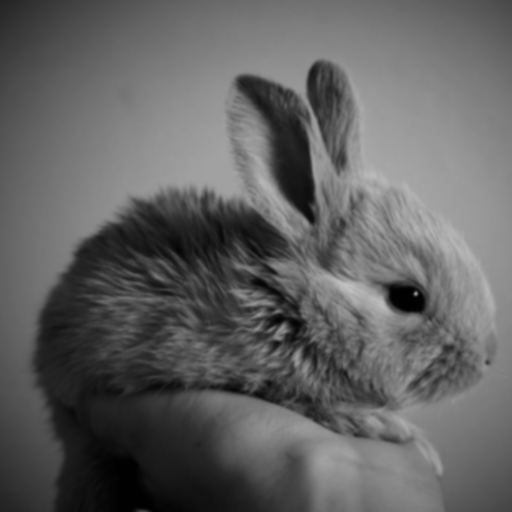
\includegraphics[width=.9\linewidth]{/home/loli/Documents/Workspace/Haskell/Class/531/eecs531-jxo136/Assignment2/data/Convolved/DCT/test2.png}
\end{itemize}
\item \texttt{y <- testDiffDct False "./data/bunny.png" \_} \\
\begin{itemize}
\item "difference in the DCT 2702.16509984095"
\item "difference in the NormalPlane 39.963790639071824"
\item 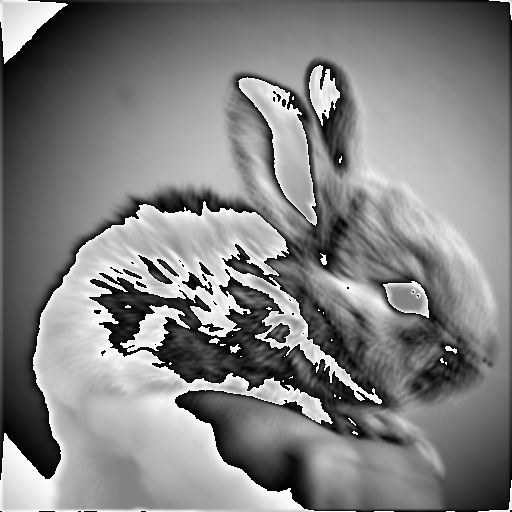
\includegraphics[width=.9\linewidth]{/home/loli/Documents/Workspace/Haskell/Class/531/eecs531-jxo136/Assignment2/data/Convolved/DCT/test-gaus-top-left.png}
\item as we can see it just turns the dark portions of the bunny white and
is oddly connected. Also note that the image is also somewhat
blurred so it seemed the filter somewhat worked
\item As expected the difference in both planes is quite high
\end{itemize}
\item a previous iteration where Ι centered the Gaussian gave me this
\begin{itemize}
\item 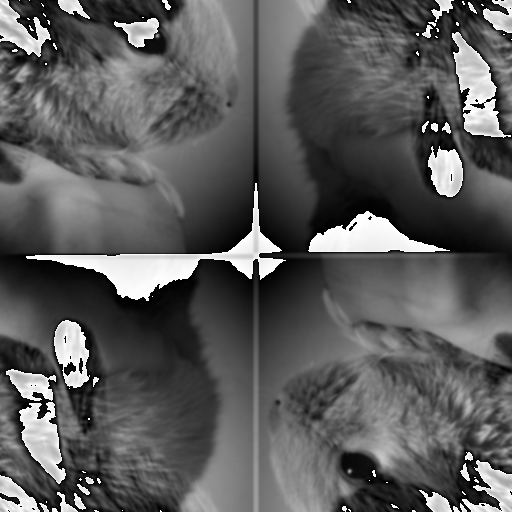
\includegraphics[width=.9\linewidth]{/home/loli/Documents/Workspace/Haskell/Class/531/eecs531-jxo136/Assignment2/data/Convolved/DCT/test-gaus-middled.png}
\item Which implies that multiplication of the DCT doesn't give anywhere
near close to being the same as the convolution. Which is expected
since we are not using the Fourier Transfomer
\end{itemize}
\item \texttt{y <- testDiffFft "./data/bunny.png" \_}
\begin{itemize}
\item I'm going to post 3 different versions of this, one with 0 bits
shifted to the right and down, 2 bits and 3 bits
\item so with two pixels shifted we get
\item 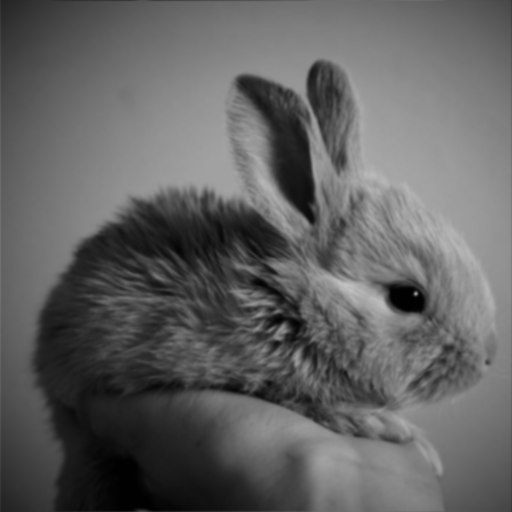
\includegraphics[width=.9\linewidth]{/home/loli/Documents/Workspace/Haskell/Class/531/eecs531-jxo136/Assignment2/data/Convolved/DCT/test-2-offset.png}
\begin{verbatim}
"difference in the DCT 1385.7172620319634 :+ 0.0"
"difference in the NormalPlane 0.1172603668112668"
\end{verbatim}
\item We can see that the difference in the normal plane is 0.11
\item And we can see that the image is wrapped around a bit on the top and
a bit on the left and right but overall the image is the exactly the same
\item this type of error would skyrocket the difference which would be
much much lower (the given python code was E-32)
\item With 3 pixels shifted we get
\item 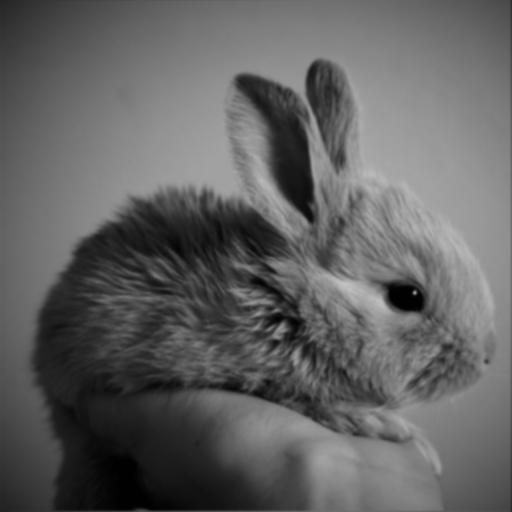
\includegraphics[width=.9\linewidth]{/home/loli/Documents/Workspace/Haskell/Class/531/eecs531-jxo136/Assignment2/data/Convolved/DCT/test-3-offset.png}
\begin{verbatim}
"difference in the DCT 1385.7172620319634 :+ 0.0"
"difference in the NormalPlane 2.411222994281215"
\end{verbatim}
\item And we can see that the image is wrapped around a bit on the far
right side and a bit on the bottom
\item The difference is greater, which implies that it's closer to being
2 pixels shifted than 3
\item 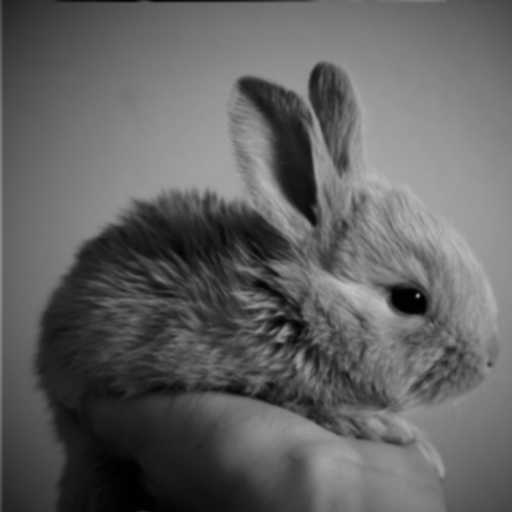
\includegraphics[width=.9\linewidth]{/home/loli/Documents/Workspace/Haskell/Class/531/eecs531-jxo136/Assignment2/data/Convolved/DCT/test-no-offset.png}
\begin{itemize}
\item This is the image with no offset after the FFT, here we can see
clearly how it is shifted.
\end{itemize}
\end{itemize}
\end{itemize}
% Emacs 25.3.1 (Org mode 8.2.10)
\end{document}